\documentclass[man]{apa2}
\usepackage{pslatex}
\usepackage{amssymb}
\usepackage{graphicx}
\usepackage{color}
\usepackage{covington}
\usepackage[usenames,dvipsnames]{xcolor}
\usepackage{booktabs}
\usepackage{setspace}

\title{The trouble with quantifiers: Children's difficulty with scalar terms extends beyond the realm of implicatures}

\threeauthors{Alexandra C. Horowtiz}{Rose M. Schneider}{Michael C. Frank}
\threeaffiliations{Department of Psychology, Stanford University}{Department of Psychology, Stanford University}{Department of Psychology, Stanford University}

\abstract{Both production and comprehension of language often require speakers and listeners to make pragmatic inferences beyond the literal sense of the utterance, particularly in the case of pragmatic implicatures. Adult listeners quickly and easily infer from the utterance ``\textit{Some} of these cookies are oatmeal raisin'' that the other cookies might be chocolate chip. On the other hand, children have more difficulty with this statement; previous research has suggested that children succeed in making implicatures in some cases but not others. However, children's performance varies tremendously across studies and tasks, limiting the number of possible direct comparisons between datasets. To address this issue, we designed a novel experimental paradigm, which both minimized task demands for participants, and enabled comparisons across different tasks. In Experiment 1, we used this paradigm to explore children's ability to compute both ad-hoc (contextual) and scalar (quantifier) implicatures, and found that while older 4-year-olds performed at ceiling for ad-hoc descriptions, they still performed poorly with scalar descriptions. In Experiment 2, we attempted to isolate children's sources of difficulty with these terms by including only scalar trials, and found that while performance increased, it was still low. Particularly, we observed a positive correlation between performance with the scalar terms ``some'' and ``none''. In Experiment 3, we explored possible sources of developmental difficulty in this task, combining our paradigm with tests of inhibitory control and quantifier knowledge. After controlling for age, we found that inhibitory control did not predict the ability to make scalar implicatures, but that children who had difficulty with ``some'' and ``none'' in an implicature task also had issues with these scalar terms in the quantifier knowledge task. Taken together, our results provide easily comparable developmental data on the development of pragmatic implicatures, and suggest that sources of difficulty over this development are not confined to making implicatures, but may be affected by quantifier knowledge and other pragmatic and processing demands.
~\\

Keywords: communication, lexicon, language evolution}

\shorttitle{The trouble with quantifiers}
\rightheader{The trouble with quantifiers}

\acknowledgements{ We gratefully acknowledge. 

~\\

\noindent Address all correspondence to Rose M. Schneider, Stanford University, Department of Psychology, Jordan Hall, 450 Serra Mall (Bldg. 420), Stanford, CA, 94305. Phone: 650-721-9270. E-mail: \texttt{rschneid@stanford.edu}.}

\begin{document}

\maketitle               

\section{Introduction}
Why are implicatures important? 

What are the developmental differences?

Why is this interesting?

What are some of the sources of difficulty with children understanding implicatures? 

Stiller et al. 

Previous studies examine implicatures using differing methods, and the results are difficult to compare

Introduce new paradigm for adhoc and scalar implicature research 


\subsection{Previous work}

In study 1,  one paradigm provides reliable and consistent measurement of implicature performance in children 3-5; however, children succeed with ad hocs, but have difficulty with scalar items; given that children were successful in computing ad hoc implicatures with this paradigm, could the poor performance in these scalar trials be due to the fact that the trials were intermixed with the adhoc trials?

In study 2, we examined this possibility by only testing scalar items, and found that while this increased performance for older children, children were still having difficulty with this task, particularly with the ``some'' and ``none'' trials

Children who had problems with ``some'' were also more likely to have issues with ``none'' 

There are several reasons we might have seen the results that we did

Children may need to know both ends of the quantifier scale in order to be able to make an implicature

There might be problems with inhibition; children in these trials might listening through the quantifier and answering purely based on the target noun; this is supported by the fact that children reliably choose ?all? for ``some'' and ``none'' trials

Do children not know what these quantifiers mean?

In study three, we explored these alternatives by running children on both the SI task, an inhibitory control task (DCCS) as well as the Give-Quantifier task, a productive measure of quantifier knowledge

Interestingly, we found that the patterns of performance persist in SI as in Horowitz and Frank, and that DCCS was not predictive of performance in either SI or GQ when controlled for age

However, we found correlations between the Give-Quantifier task with ?some? and ?none? trials (except for GQ none and SI some, I think) when controlling for age; this seems to indicate that difficulties with these scalar terms exist outside of the implicature realm

Children just seem to have a trouble with quantifiers


\section{Experiment 1: Ad hoc and scalar implicature computation in children}

Given the difficulty in equating results on children's computation of implicatures across different methods and paradigms, we created a single task that could be adapted to investigate both ad hoc and scalar items in one task. This task involved one set of stimuli presented in the same order to all participants; however, the particular items queried were counterbalanced across participants. Thus, with one set of stimuli we created a novel paradigm wherein we could directly compare children's performance on both ad hoc and scalar implicatures in a single experimental session. In Experiment 1, we included questions about ad hoc and scalar implicatures within one session, and found that this paradigm was appropriate for ad hoc items, but children still experienced difficulty computing scalar items.

% In Experiment 2, we included only scalar items in the task, and found that participants were moderately more successful at making implicatures when these trials were presented in isolation. In Experiment 3, we explored two alternatives potentially driving children's difficulties in this task.  

\subsection{Methods}

\subsubsection{Participants} A planned sample of 48 children was recruited from Bing Nursery School at Stanford University. These children were drawn from two age groups: twenty-four 4.0 -- 4.5-year-olds (M = 4;2, median = 4.19, SD = 0.14) and 24 4.5 -- 5.0-year-olds (M = 4.74, median = 4.73, SD = .16). Two children were excluded from the final sample for not completing the task, and one additional child was excluded due to experimenter error. The final sample was comprised of (XX males and XX females) with English as their primary language. Across all experiments, no child completed more than one session of the task. 

\begin{figure} 
 \begin{center} 
  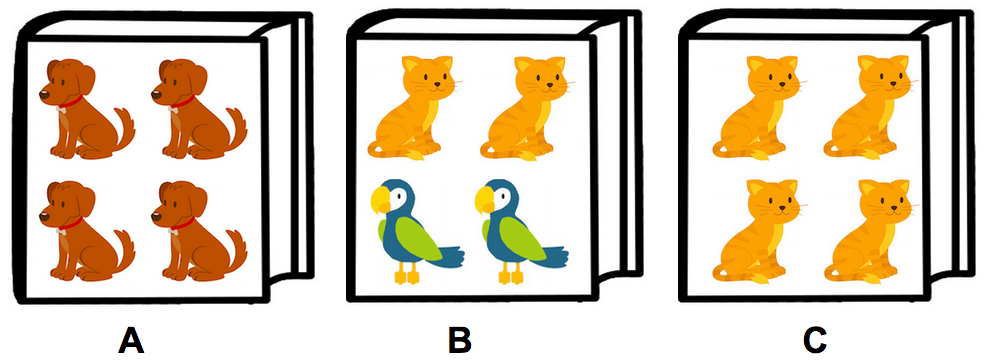
\includegraphics[height=2in]{figures/implicatures_demo_letters.png} 
  \caption{\label{fig:demo} Example trial stimuli used in all experiments. Children received a clue from the experimenter about which book she had in mind and responded based solely on the clue; this was either an ad hoc or a scalar description of a book with either an unambiguous or implicature target.} 
 \end{center} 
\end{figure}	 

\subsubsection{Stimuli}
Stimuli for all experiments were created to be appropriate for questions about both ad hoc and scalar implicatures, allowing the experimenter to use one set of stimuli for both kinds of items in one experimental session. The experimental stimuli consisted of a set of printed pictures of three book covers with four familiar items on each cover. In each trial, one book cover contained four items of the same kind (e.g., four cats), another book cover contained four items of another kind (e.g., dogs), and the final cover contained two items of a new set and two items repeated from one of the other book covers (e.g., two birds and two cats). An example of the stimuli can be seen in Figure \ref{fig:demo}. Experiment 1 consisted of 18 test trials preceded by one test trial, with three book covers containing only one familiar item. All items on the book covers were familiar to children, and were able to be identified. All participants saw the same book covers in the same order. 


\subsubsection{Procedure}
Participants were tested in individual sessions in a quiet room at their nursery school. The experimenter introduced the study as a guessing game, and explained that the child would receive a hint about which book cover the experimenter had in mind. In the instructions for the task, the experimenter emphasized that the child would only receive one clue about what book the experimenter was describing, and they had to use that clue to make their decision. All participants saw the same book covers in the same order; however, (three?) scripts with both ad-hoc and scalar trials were counterbalanced across participants. A breakdown of trial types and sample scripts can be seen in (Table 1). 

Prior to the test trials, children were familiarized to the task with a practice trial. The practice trial consisted of three book covers, each displaying a single unique and familiar item. After children had successfully completed the practice, children saw 18 test trials with stimuli of books containing sets of familiar items. At the start of every trial, the experiment would provide the child with either an ad-hoc or scalar description of one of the books and instruct the child to point to the book she was describing. If the child pointed to more than one book, or the response was otherwise ambiguous, the experimenter emphasized again that she was talking about just one book, and that they should choose the single book she was describing. 

In ad-hoc trials (eight total), the experimenter's descriptions of the target book used names of the pictured objects, providing contextual support for the target. Ad-hoc control trials referred to an unambiguous target (e.g., ``On the cover of my book, there are dogs'' in Figure \ref{fig:demo}). while implicature trials required the child to reason about the speaker's meaning given the ambiguous utterance (e.g., ``On the cover of my book, there are cats'', which could refer to either the book containing only cats or the book containing cats and birds). In these critical trials, children had to understand that the speaker could potentially be talking about either the book with four or two of the named object, but that by opting to describe only one kind of object she was referring to the cover with four of the same object; otherwise, she would have mentioned both kinds of objects, or the ones unique to that cover (i.e., birds). 

In scalar trials (ten total), the experimenter described the target book with quantifiers. For scalar items, control trials referred to unambiguous targets with the quantifiers ``all'' and ``none'' (e.g., ``On the cover of my book, \textit{all/none} of the pictures are cats'') or an unambiguous referent of ``some'' (e.g., ``On the cover of my book, \textit{some} of the pictures are birds''). On critical scalar implicature trials, the experimenter used the weak quantifier ``some'' to reference the item pictured across two book covers (e.g., ``On the cover of my book, \textit{some} of the pictures are cats''). These trials required the child to reason that because the speaker used the weak quantifier ``some'', some must be referring to the book picturing only two of the named target, or else she would have used the strong quantifier ``all''. 

All participants saw image sets in the same order; however, these image sets were counterbalanced for target location and book triad position. Description condition and trial-type were further randomized across participants, and were spaced to avoid immediate repeat trial types. Children did not receive feedback after the test trial.

\subsection{Results and Discussion}



\section{Experiment 2: Mapping Task (Artificial Objects)}


\subsection{Methods}
\subsubsection{Participants} 
\subsubsection{Stimuli}

\subsubsection{Procedure}


\subsection{Results and Discussion}

				
\section{Experiment 3: Control Mapping Task (Artificial Objects)}

\subsection{Methods}
\subsubsection{Participants} 200 participants completed the experiment.
\subsubsection{Stimuli} h

\subsubsection{Procedure}
h

\subsection{Results and Discussion}
h

\section{General Discussion}

h




\bibliographystyle{apacite2}
\bibliography{biblibrary}

\newpage
\theappendix 

\section{}

\end{document}